\documentclass[10pt]{beamer}
\usepackage[english]{babel}
\usepackage[utf8]{inputenc}
\usepackage[T1]{fontenc}
\usepackage{helvet}

%-------------------------------------------------------
% INFORMATION IN THE TITLE PAGE
%-------------------------------------------------------

\newcommand{\cstitle}{\textbf{Bioinformatics}}
\subtitle[]{An Analysis of k-Mer Frequency Features with Machine Learning Models for Viral Subtyping Classification}
\newcommand{\cscourseCode}{1005155}
\newcommand{\csauthor}{MSc. Vicente Machaca Arceda}
\institute[UNSA]{Universidad La Salle}
\newcommand{\csemail}{vmachacaa@ulasalle.edu.pe}
\newcommand{\instituteabr}{Salle}
\newcommand{\nameUp}{}
\date{2020}
\title[\cscourseCode]{\cstitle}
\author{\csauthor}
%%%%%%%%%%%%%%%%%

%-------------------------------------------------------
% CHOOSE THE THEME
%-------------------------------------------------------
\def\mycmd{0} % CS THEME
%\def\mycmd{1} % MYTHEME
%-------------------------------------------------------

\if\mycmd1
	\usetheme[]{Feather}
	\newcommand{\chref}[2]{	\href{#1}{{\usebeamercolor[bg]{Feather}#2}} }
\else
	\usepackage{csformat}
	\newcommand{\chref}[3][blue]{\href{#2}{\color{#1}{#3}}}%
\fi

\newcommand{\1}{
        	\setbeamertemplate{background}{
        		
\includegraphics[width=\paperwidth,height=\paperheight]{img/1}
        		\tikz[overlay] \fill[fill opacity=0.75,fill=white] (0,0) rectangle (-\paperwidth,\paperheight);
        	}
}



%-------------------------------------------------------
% THE BODY OF THE PRESENTATION
%-------------------------------------------------------

\begin{document}


\AtBeginSubsection[]
{
    \begin{frame}
        \frametitle{Tabla de contenido}
        \tableofcontents[currentsubsection]
    \end{frame}
}


%-------------------------------------------------------
% THE TITLEPAGE
%-------------------------------------------------------

\if\mycmd1 % MY THEME
	\1{
	\begin{frame}[plain,noframenumbering] 
		\titlepage 
	\end{frame}}

\else % CS THEME
	\maketitle
\fi


%-------------------------------------------------------
%-------------------------------------------------------
%\begin{frame}{Overview}
%	\tableofcontents
%\end{frame}
%-------------------------------------------------------
%-------------------------------------------------------



%%%%%%%%%%%%%%%%%%%%%%%%%%%%%%%%%%%%%%%%%%%%%%%%%%%%%%%%
\section{Introduction}
%%%%%%%%%%%%%%%%%%%%%%%%%%%%%%%%%%%%%%%%%%%%%%%%%%%%%%%%

%%%%%%%%%%%%%%%%%%%%%%%%%%%%%%%%%%%%%%%%%%%%%%%%%%%%%%%%
%\subsection{The purpose of Bioinformatics}
%%%%%%%%%%%%%%%%%%%%%%%%%%%%%%%%%%%%%%%%%%%%%%%%%%%%%%%%


%-------------------------------------------------------
%-------------------------------------------------------
%\begin{frame}{The purpose of Bioinformatics}{Why a person has cancer?}
%	\begin{figure}[]
%		\centering
%		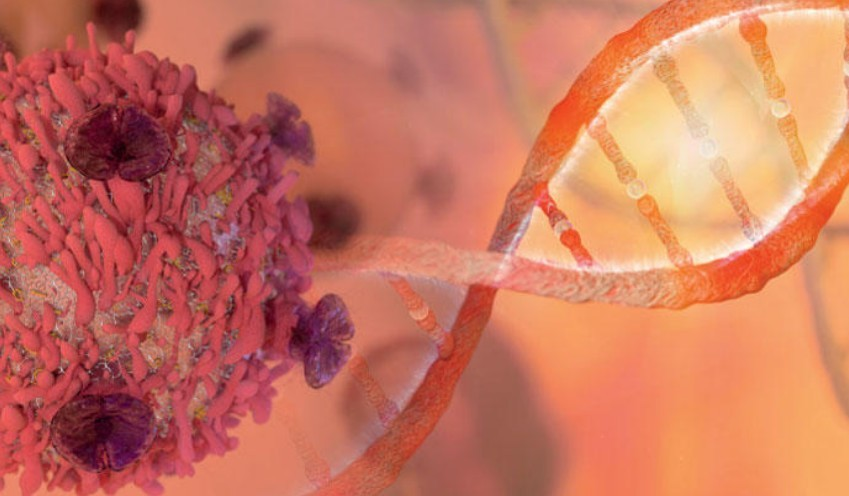
\includegraphics[width=\textwidth,height=0.6\textheight,keepaspectratio]{img/mot3.jpg}
%		\label{img:mot2}
%		\caption{Why a person has cancer?}
%	\end{figure}
%\end{frame}
%-------------------------------------------------------
%-------------------------------------------------------

%-------------------------------------------------------
%-------------------------------------------------------
%\begin{frame}{The purpose of Bioinformatics}{Why some medicines no work in some persons?}
%	\begin{figure}[]
%		\centering
%		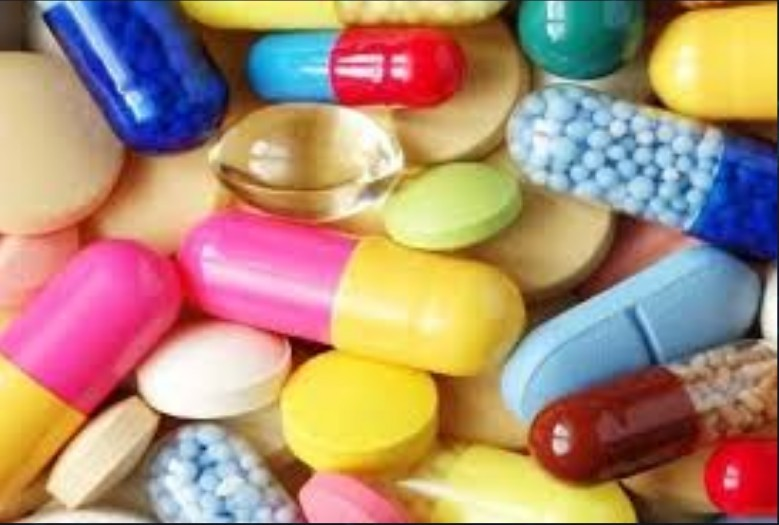
\includegraphics[width=\textwidth,height=0.6\textheight,keepaspectratio]{img/mot4.jpg}
%		\label{img:mot2}
%		\caption{Why some medicines no work in some persons?}
%	\end{figure}
%\end{frame}
%-------------------------------------------------------
%-------------------------------------------------------

%-------------------------------------------------------
%-------------------------------------------------------
%\begin{frame}{The purpose of Bioinformatics}{Treatment Development}
%	\begin{figure}[]
%		\centering
%		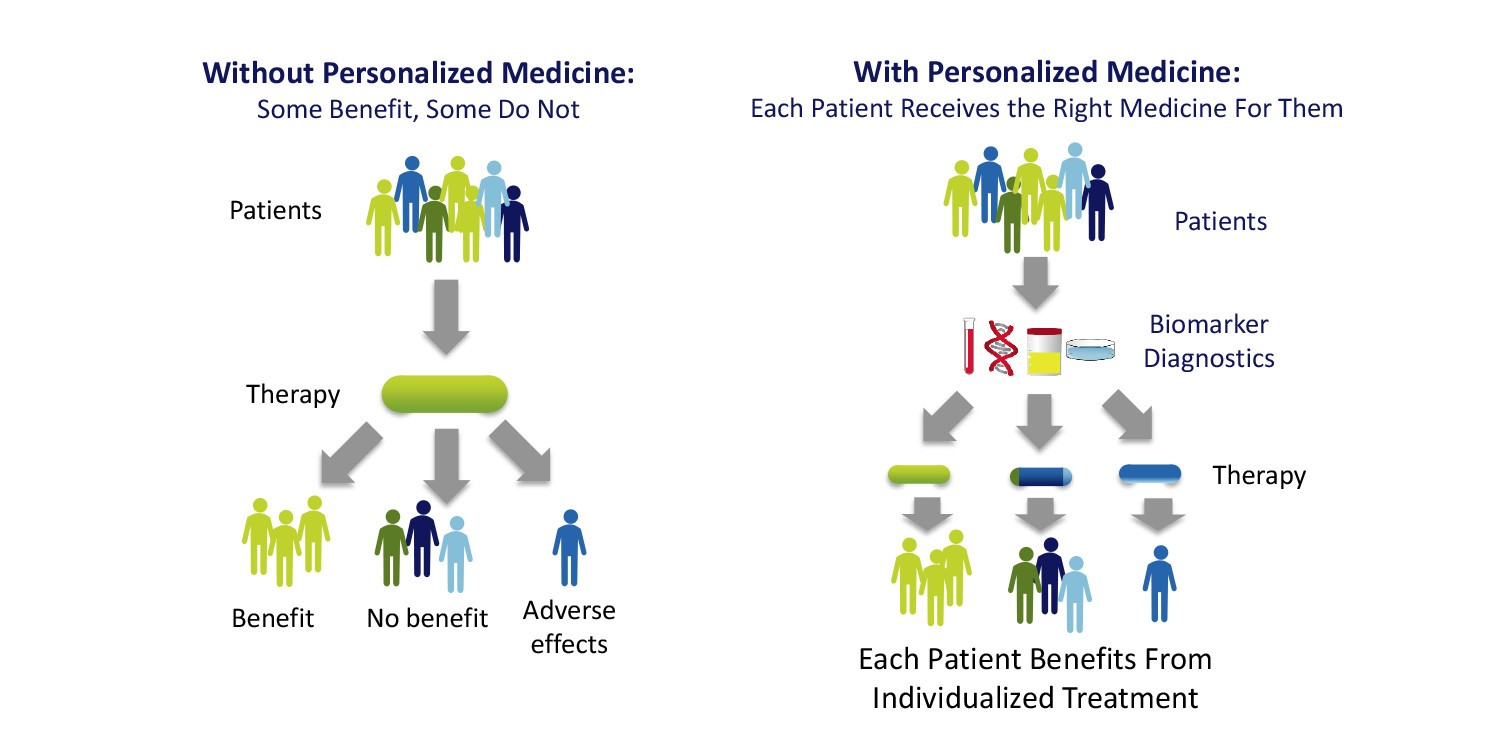
\includegraphics[width=\textwidth,height=0.7\textheight,keepaspectratio]{img/mot5.jpg}
%		\label{img:mot2}
%		\caption{Personalized Medicine: New Approach to Treatment of Disease}
%	\end{figure}
%\end{frame}
%-------------------------------------------------------
%-------------------------------------------------------

%-------------------------------------------------------
%-------------------------------------------------------
%\begin{frame}{The purpose of Bioinformatics}{Protein structure prediction}
%	\begin{figure}[]
%		\centering
%		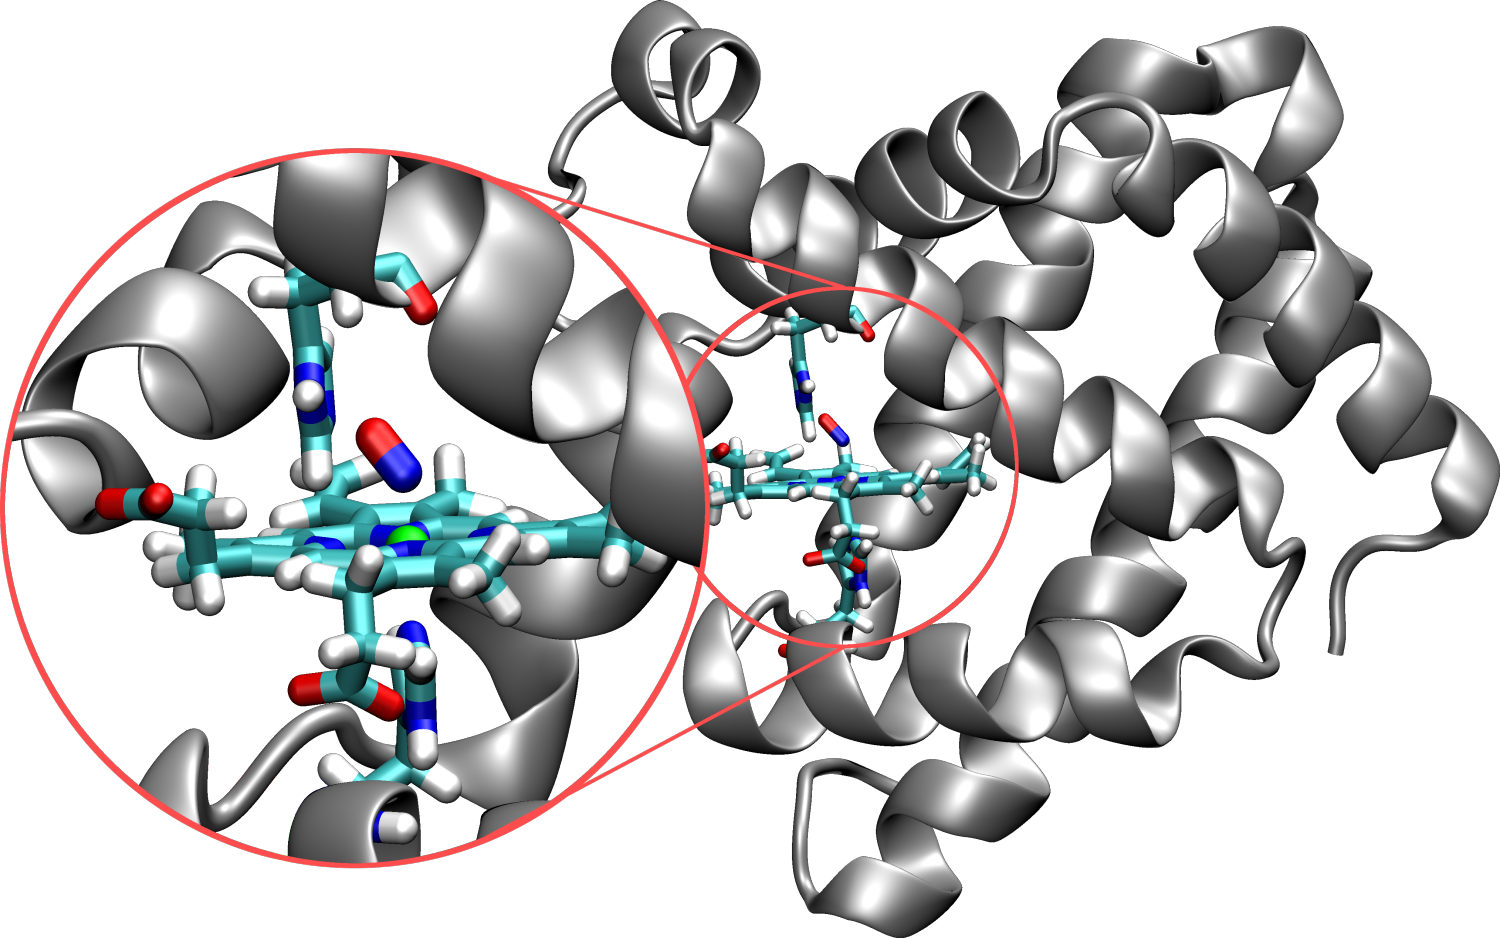
\includegraphics[width=\textwidth,height=0.7\textheight,keepaspectratio]{img/protein2}
		%https://www.pngwing.com/en/free-png-mrxlb
%		\label{img:mot2}
%		\caption{Computer simulation of protein-ligand.}
%	\end{figure}
%\end{frame}
%-------------------------------------------------------
%-------------------------------------------------------



%%%%%%%%%%%%%%%%%%%%%%%%%%%%%%%%%%%%%%%%%%%%%%%%%%%%%%%%
\subsection{What is Bioinformatics?}
%%%%%%%%%%%%%%%%%%%%%%%%%%%%%%%%%%%%%%%%%%%%%%%%%%%%%%%%

%-------------------------------------------------------
%-------------------------------------------------------
\begin{frame}{Introduction}{What is Bioinformatics?}
	
	According to Luscombe et al.: \textbf{Bioinformatics} involves the technology that uses computers for storage, retrieval, manipulation, and distribution of information related to biological macromolecules such as DNA, RNA, and proteins \cite{luscombe2001bioinformatics}.
	
\end{frame}
%-------------------------------------------------------
%-------------------------------------------------------


%-------------------------------------------------------
%-------------------------------------------------------
\begin{frame}{Bioinformatics}
	\begin{figure}[]
		\centering
		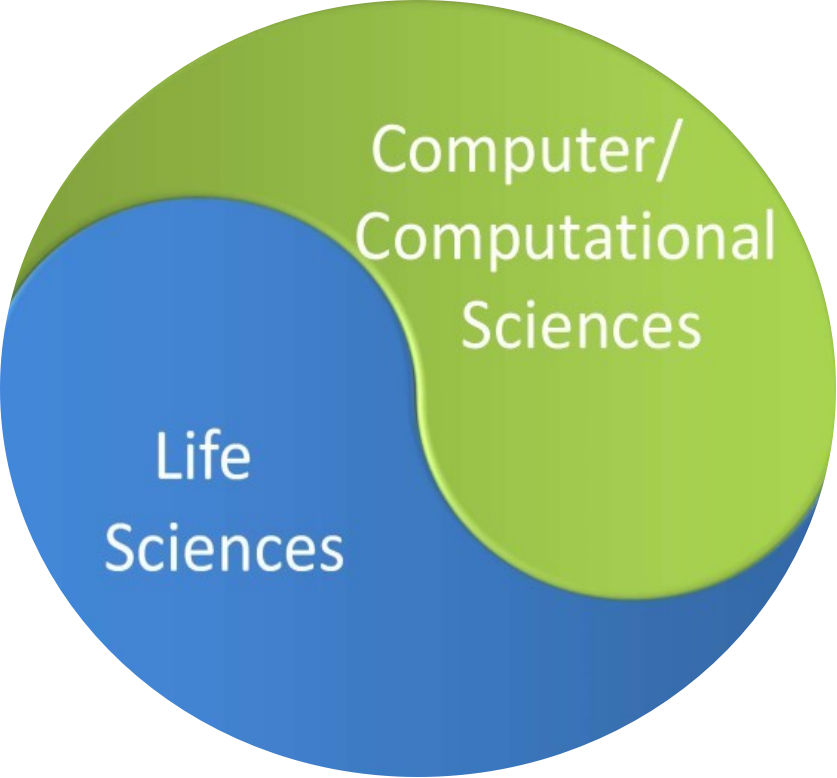
\includegraphics[width=\textwidth,height=0.7\textheight,keepaspectratio]{img/kmer/bio2.png}
		\label{img:mot2}
		%\caption{Computer simulation of protein-ligand.}
	\end{figure}
\end{frame}
%-------------------------------------------------------
%-------------------------------------------------------

%-------------------------------------------------------
%-------------------------------------------------------
\begin{frame}{Bioinformatics}
	\begin{figure}[]
		\centering
		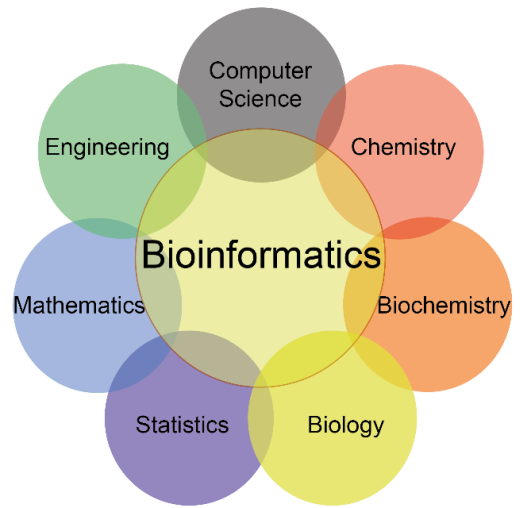
\includegraphics[width=\textwidth,height=0.7\textheight,keepaspectratio]{img/kmer/bio4}
		\label{img:mot2}
		%\caption{Computer simulation of protein-ligand.}
	\end{figure}
\end{frame}
%-------------------------------------------------------
%-------------------------------------------------------



%%%%%%%%%%%%%%%%%%%%%%%%%%%%%%%%%%%%%%%%%%%%%%%%%%%%%%%%%%%%%%%%%%%%%%%%%%%%%%%%%%%%%%%%%%%%%%%%%%%%%%%%%%%%%%%%
%%%%%%%%%%%%%%%%%%%%%%%%%%%%%%%%%%%%%%%%%%%%%%%%%%%%%%%%%%%%%%%%%%%%%%%%%%%%%%%%%%%%%%%%%%%%%%%%%%%%%%%%%%%%%%%%
%%%%%%%%%%%%%%%%%%%%%%%%%%%%%%%%%%%%%%%%%%%%%%%%%%%%%%%%%%%%%%%%%%%%%%%%%%%%%%%%%%%%%%%%%%%%%%%

%%%%%%%%%%%%%%%%%%%%%%%%%%%%%%%%%%%%%%%%%%%%%%%%%%%%%%%%
\section{Viral subtype classification}
%%%%%%%%%%%%%%%%%%%%%%%%%%%%%%%%%%%%%%%%%%%%%%%%%%%%%%%%

%%%%%%%%%%%%%%%%%%%%%%%%%%%%%%%%%%%%%%%%%%%%%%%%%%%%%%%%
\subsection{Viral subtype}
%%%%%%%%%%%%%%%%%%%%%%%%%%%%%%%%%%%%%%%%%%%%%%%%%%%%%%%%

%-------------------------------------------------------
%-------------------------------------------------------
\begin{frame}{Viral subtype classification}{Subtype of HIV}
	\begin{figure}[]
		\centering
		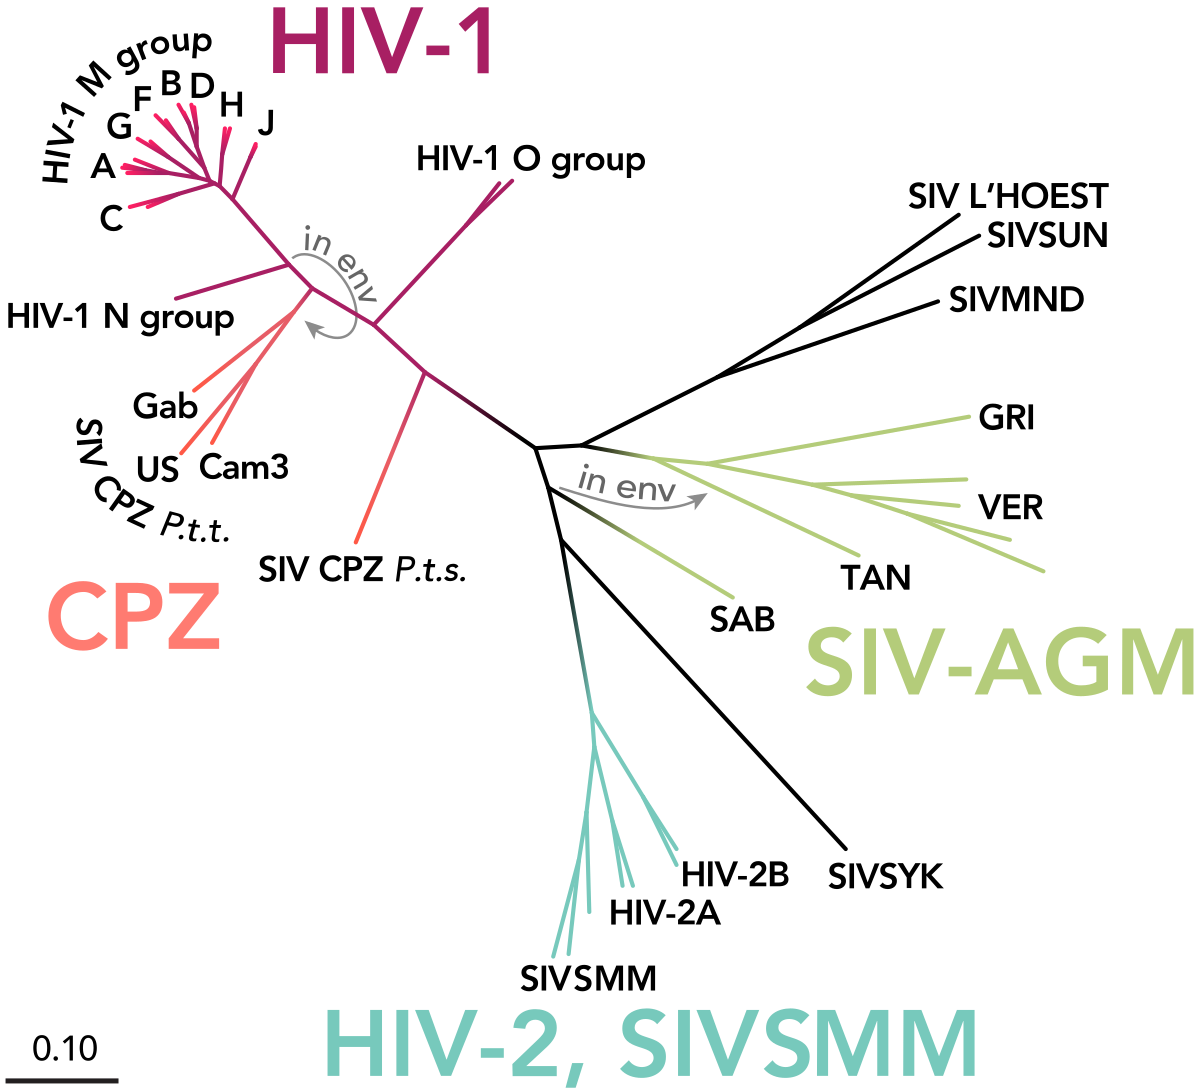
\includegraphics[width=\textwidth,height=0.6\textheight,keepaspectratio]{img/kmer/HIV}
		\label{img:mot2}
		\caption{Phylogenetic tree of the SIV and HIV viruses. Source: \cite{hivwiki2020}}
	\end{figure}
\end{frame}
%-------------------------------------------------------
%-------------------------------------------------------

%-------------------------------------------------------
%-------------------------------------------------------
\begin{frame}{Viral subtype classification}{Example of DNA}
	\begin{figure}[]
		\centering
		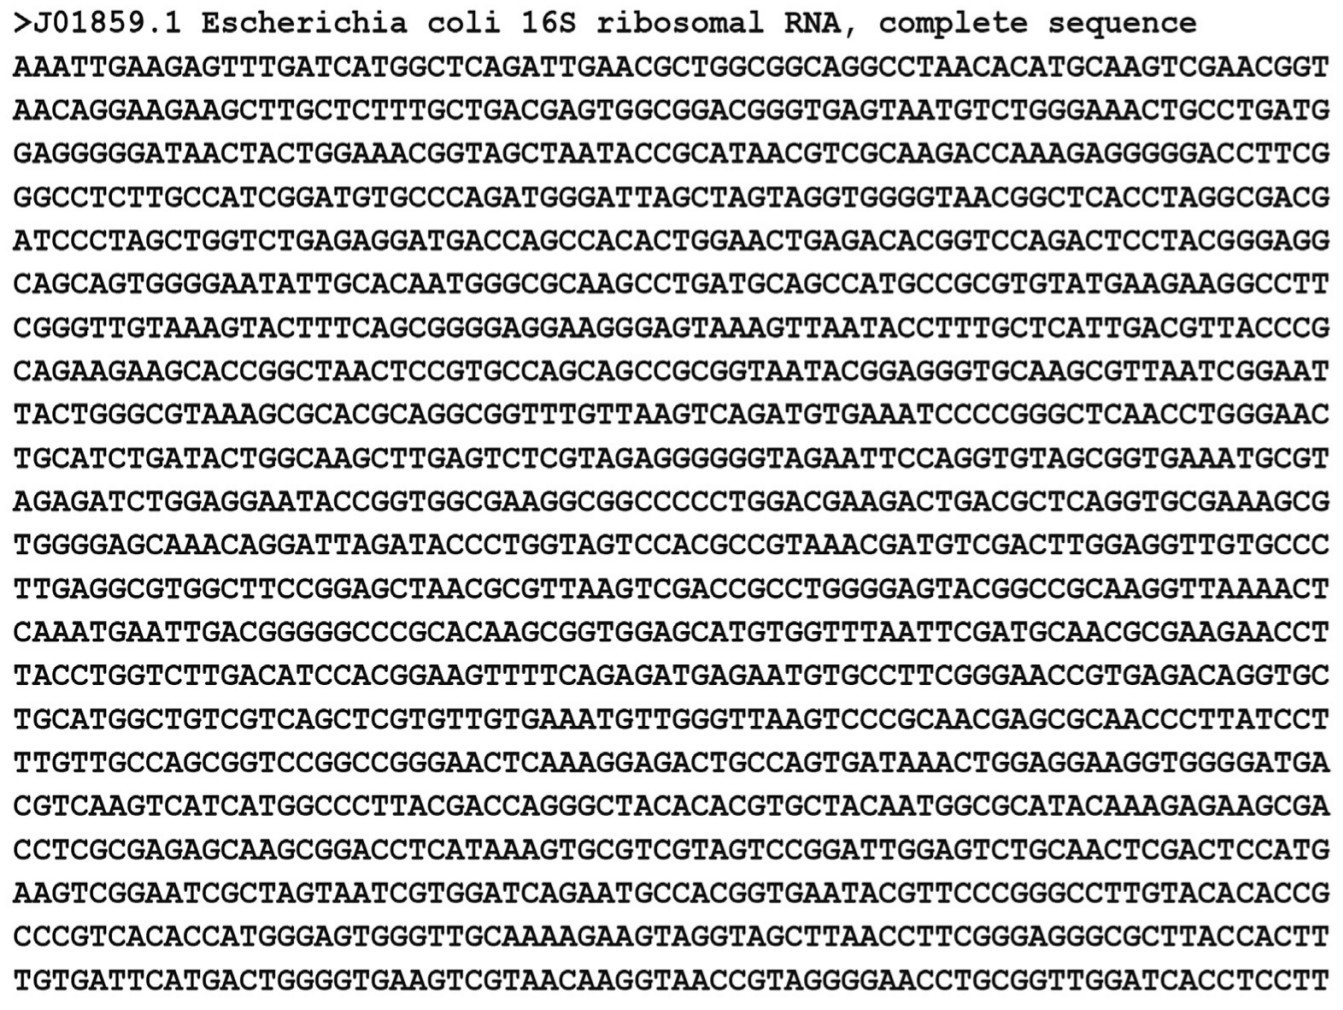
\includegraphics[width=\textwidth,height=0.7\textheight,keepaspectratio]{img/kmer/dnaimg_1}
		\label{img:mot2}
		%\caption{Computer simulation of protein-ligand.}
	\end{figure}
\end{frame}
%-------------------------------------------------------
%-------------------------------------------------------


%-------------------------------------------------------
%-------------------------------------------------------
\begin{frame}{Viral subtype classification}{Problem}
	\begin{block}{}
		\begin{itemize}
			\item The most used \textbf{alignment-based} method are BLAST and CLUSTALW. \pause
			\item They are slow. For example, it take one hour to align 18 sequences of 18k bp. \pause
			\item DNA sequences increases every day, so \textbf{alignment-based} methods get slower every second.
		\end{itemize}
	\end{block}
\end{frame}
%-------------------------------------------------------
%-------------------------------------------------------

%-------------------------------------------------------
%-------------------------------------------------------
\begin{frame}{Viral subtype classification}{Objective}
	\begin{block}{}
		Compare  \textbf{alignment-free} algorithms based on k-mer frequencies. 
		\begin{itemize}
			\item Kameris  \cite{solis2018open}.
			\item Castor-KRFE  \cite{lebatteux2019toward}.
			\item CNN.
		\end{itemize}
	\end{block}

	\begin{block}{}
		 We got two publications \cite{arceda2020analysis},  \cite{machaca2020analysis}.
	\end{block}
	
\end{frame}
%-------------------------------------------------------
%-------------------------------------------------------


%%%%%%%%%%%%%%%%%%%%%%%%%%%%%%%%%%%%%%%%%%%%%%%%%%%%%%%%%%%%%%%%%%%%%%%%%%%%%%%%%%%%%%%%%%%%%%%%%%%%%%%%%%%%%%%%
%%%%%%%%%%%%%%%%%%%%%%%%%%%%%%%%%%%%%%%%%%%%%%%%%%%%%%%%%%%%%%%%%%%%%%%%%%%%%%%%%%%%%%%%%%%%%%%%%%%%%%%%%%%%%%%%
%%%%%%%%%%%%%%%%%%%%%%%%%%%%%%%%%%%%%%%%%%%%%%%%%%%%%%%%%%%%%%%%%%%%%%%%%%%%%%%%%%%%%%%%%%%%%%%

%%%%%%%%%%%%%%%%%%%%%%%%%%%%%%%%%%%%%%%%%%%%%%%%%%%%%%%%
\subsection{K-mer frequency}
%%%%%%%%%%%%%%%%%%%%%%%%%%%%%%%%%%%%%%%%%%%%%%%%%%%%%%%%

%-------------------------------------------------------
%-------------------------------------------------------
\begin{frame}{K-mer frequency}{k-mer}
	\begin{block}{}
		For sequence  $s = \{ A,C,T,G,A,C \}$
	\end{block}
	
	\begin{block}{}
		\begin{itemize}
			\item 2-mers set: $\{ AC, CT, TG, GA \}$  $\rightarrow$ $\{ 2, 1, 1, 1 \}$
			\item 3-mers set: $\{ ACT, CTG, TGA, GAC \}$	$\rightarrow$ $\{ 1, 1, 1, 1 \}$			 	
		\end{itemize}
	\end{block}	
\end{frame}
%-------------------------------------------------------
%-------------------------------------------------------

%%%%%%%%%%%%%%%%%%%%%%%%%%%%%%%%%%%%%%%%%%%%%%%%%%%%%%%%
\subsection{Kameris}
%%%%%%%%%%%%%%%%%%%%%%%%%%%%%%%%%%%%%%%%%%%%%%%%%%%%%%%%

%-------------------------------------------------------
%-------------------------------------------------------
\begin{frame}{Kameris}{K-mer frequency}
	\begin{figure}[h]
		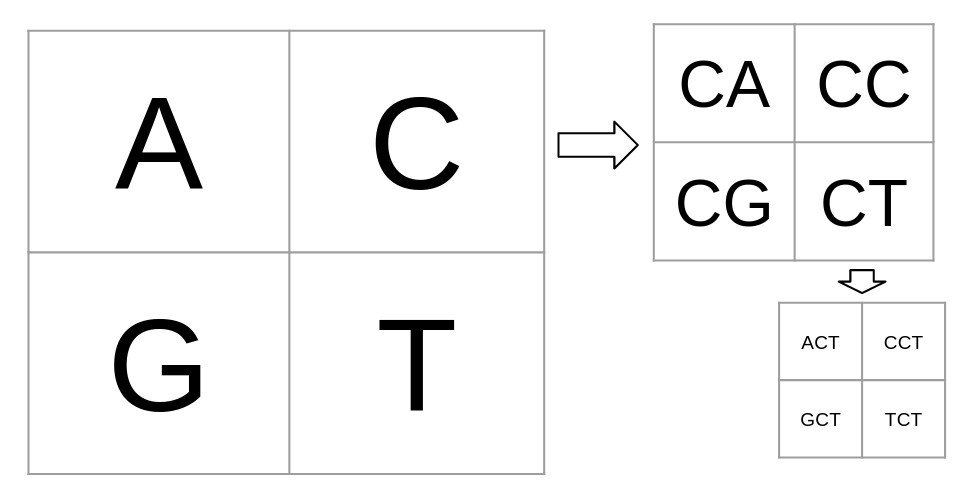
\includegraphics[width=0.8\textwidth]{img/kmer/cgr.jpg}
		%\caption{A FCGR matrix. The \textit{G} quadrant sub-divided into the corresponding G-endings and the \textit{TG} quadrant sub-divided into the corresponding \textit{TG-endings}. \cite{pandit2010using}}
		\caption{A FCGR matrix. The \textit{G} quadrant sub-divided into the corresponding G-endings and the \textit{TG} quadrant sub-divided into the corresponding \textit{TG-endings}.}
		\label{fig:cgr}
	\end{figure}
\end{frame}
%-------------------------------------------------------
%-------------------------------------------------------

%-------------------------------------------------------
%-------------------------------------------------------
\begin{frame}{Kameris}{K-mer frequency}
	\begin{figure}[h]
		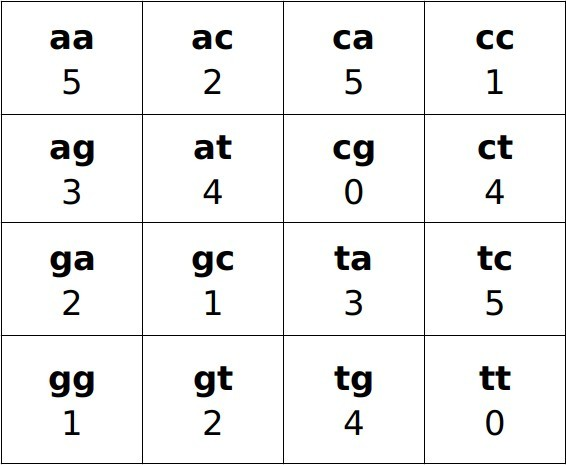
\includegraphics[width=0.6\textwidth]{img/kmer/cgr4.jpg}
		\caption{A FCGR k-mer example, each k-mer is representing as a cell in the matrix, and the frequency of each k-mer is represented as the pixel value.}
		\label{fig:cgr3}
	\end{figure}
\end{frame}
%-------------------------------------------------------
%-------------------------------------------------------

%-------------------------------------------------------
%-------------------------------------------------------
\begin{frame}{Kameris}{Method}
	\begin{block}{}
		\begin{itemize}
			\item Compute k-mer frequencies using FCGR ($4^k$).
			\item Dimensionality reduction with Sigle Value Decomposition.
			\item SVM classifier.
		\end{itemize}
	\end{block}
\end{frame}
%-------------------------------------------------------
%-------------------------------------------------------


%%%%%%%%%%%%%%%%%%%%%%%%%%%%%%%%%%%%%%%%%%%%%%%%%%%%%%%%
\subsection{Castor-KRFE}
%%%%%%%%%%%%%%%%%%%%%%%%%%%%%%%%%%%%%%%%%%%%%%%%%%%%%%%%

%-------------------------------------------------------
%-------------------------------------------------------
\begin{frame}{Castor-KRFE}{Method}
	\begin{block}{}
		\begin{itemize}
			\item Compute k-mer frequencies, just take into account k-mer presented in DNA sequence.
			\item Feature elimination with Recursive Feature Elimination.
			\item SVM classifier.
		\end{itemize}
	\end{block}
\end{frame}
%-------------------------------------------------------
%-------------------------------------------------------

%%%%%%%%%%%%%%%%%%%%%%%%%%%%%%%%%%%%%%%%%%%%%%%%%%%%%%%%
\subsection{CNN}
%%%%%%%%%%%%%%%%%%%%%%%%%%%%%%%%%%%%%%%%%%%%%%%%%%%%%%%%

%-------------------------------------------------------
%-------------------------------------------------------
\begin{frame}{CNN}{FCGR}
		\begin{figure}[h]
		\centering
		
\includegraphics[width=0.6\textwidth]{img/kmer/HIV1_G_596_0_k=5}
		\caption{A FCGR (k=5) of a HIV-1 genome.}
		\label{fig:cgr_img}
	\end{figure}
\end{frame}
%-------------------------------------------------------
%-------------------------------------------------------

%-------------------------------------------------------
%-------------------------------------------------------
\begin{frame}{CNN}{Method}
	\begin{block}{}
		\begin{itemize}
			\item Compute FCGR 
			\item Represent the FCGR as an image.
			\item Train with CNNs.
		\end{itemize}
	\end{block}
\end{frame}
%-------------------------------------------------------
%-------------------------------------------------------

%%%%%%%%%%%%%%%%%%%%%%%%%%%%%%%%%%%%%%%%%%%%%%%%%%%%%%%%
\section{Results}
%%%%%%%%%%%%%%%%%%%%%%%%%%%%%%%%%%%%%%%%%%%%%%%%%%%%%%%%

%%%%%%%%%%%%%%%%%%%%%%%%%%%%%%%%%%%%%%%%%%%%%%%%%%%%%%%%
\subsection{Materials and methods}
%%%%%%%%%%%%%%%%%%%%%%%%%%%%%%%%%%%%%%%%%%%%%%%%%%%%%%%%

%-------------------------------------------------------
%-------------------------------------------------------
\begin{frame}{Methods used}
	\begin{table}	
		\caption{Methods used in this research.}
		\label{tab:methods}
		\begin{tabular}{lp{6.5cm}}
			\hline
			\textbf{Method name} & \textbf{Description} \\ \hline
			Kameris-SVD	& Kameris with dimensionality reduction SVD. \\
			Kameris	& Kameris without dimensionality reduction. \\
			Castor-KRFE & Castor with feature elimination RFE. \\
			Castor & Castor without feature elimination. \\
			CNN & The method that used FCGR with CNN (three architectures: CNN-1, CNN-2 and CNN-3). \\
			ML-DSP & The method that process the DNA as a digital signal. \\
			\hline
		\end{tabular}
		
		\label{tab:datasets}
	\end{table}

\end{frame}
%-------------------------------------------------------
%-------------------------------------------------------

%%%%%%%%%%%%%%%%%%%%%%%%%%%%%%%%%%%%%%%%%%%%%%%%%%%%%%%%
\subsection{Datasets}
%%%%%%%%%%%%%%%%%%%%%%%%%%%%%%%%%%%%%%%%%%%%%%%%%%%%%%%%

%-------------------------------------------------------
%-------------------------------------------------------
\begin{frame}{Datasets}
		\begin{table}[h]
		\centering
		\caption{The datasets used in the experiments.}
		\label{tab:datasets}
		\begin{tabular}{llll}
			\hline
			& Average  &   No. of & No. of    \\
			Data sets		& seq. length & classes &   instances \\
			\hline
			
			HBVGENCG    & 3189   & 8  & 230    \\
			HIVGRPCG    & 9164   & 4  & 76      \\
			HIVSUBCG    & 8992   & 18 & 597     \\
			HIVSUBPOL   & 1211   & 28 & 1352    \\
			INFSUBHA    & 1719   & 2  & 10825   \\
			INFSUBMP    & 759    & 2  & 21421   \\
			INSUBFNA    & 1416   & 2  & 10715   \\
			EBOSPECG    & 18917  & 5  & 751    \\
			RHISPECG    & 369    & 3  & 1316    \\
			HPVGENCG    & 7610   & 3  & 125     \\			
			\hline
		\end{tabular}
		
		\label{tab:datasets}
	\end{table}
	
\end{frame}
%-------------------------------------------------------
%-------------------------------------------------------


%-------------------------------------------------------
%-------------------------------------------------------
\begin{frame}{Datasets}
	\begin{table}[h]
		\centering
		\caption{The datasets used in the experiments.}
		\label{tab:datasets}
		\begin{tabular}{llll}
			\hline
			& Average  &   No. of & No. of    \\
			Data sets		& seq. length & classes &   instances \\
			\hline	
			Primates    & 16626  & 2  & 148     \\
			Dengue      & 10595  & 4  & 4721    \\
			Protists    & 31712  & 3  & 159     \\
			Fungi       & 49178  & 3  & 224     \\
			Plants      & 277931 & 2  & 174     \\
			Amphibians  & 17530  & 3  & 290    \\
			Insects     & 15689  & 7  & 898     \\
			3classes    & 16292  & 3  & 2170    \\
			Vertebrates & 16806  & 5  & 4322    \\
			\hline
		\end{tabular}
		
		\label{tab:datasets}
	\end{table}
	
\end{frame}
%-------------------------------------------------------
%-------------------------------------------------------


%%%%%%%%%%%%%%%%%%%%%%%%%%%%%%%%%%%%%%%%%%%%%%%%%%%%%%%%
\subsection{Results}
%%%%%%%%%%%%%%%%%%%%%%%%%%%%%%%%%%%%%%%%%%%%%%%%%%%%%%%%

%-------------------------------------------------------
%-------------------------------------------------------
\begin{frame}{Results}{Comparison between Kameris and Castor}
	\begin{figure}[h]
		\centering
		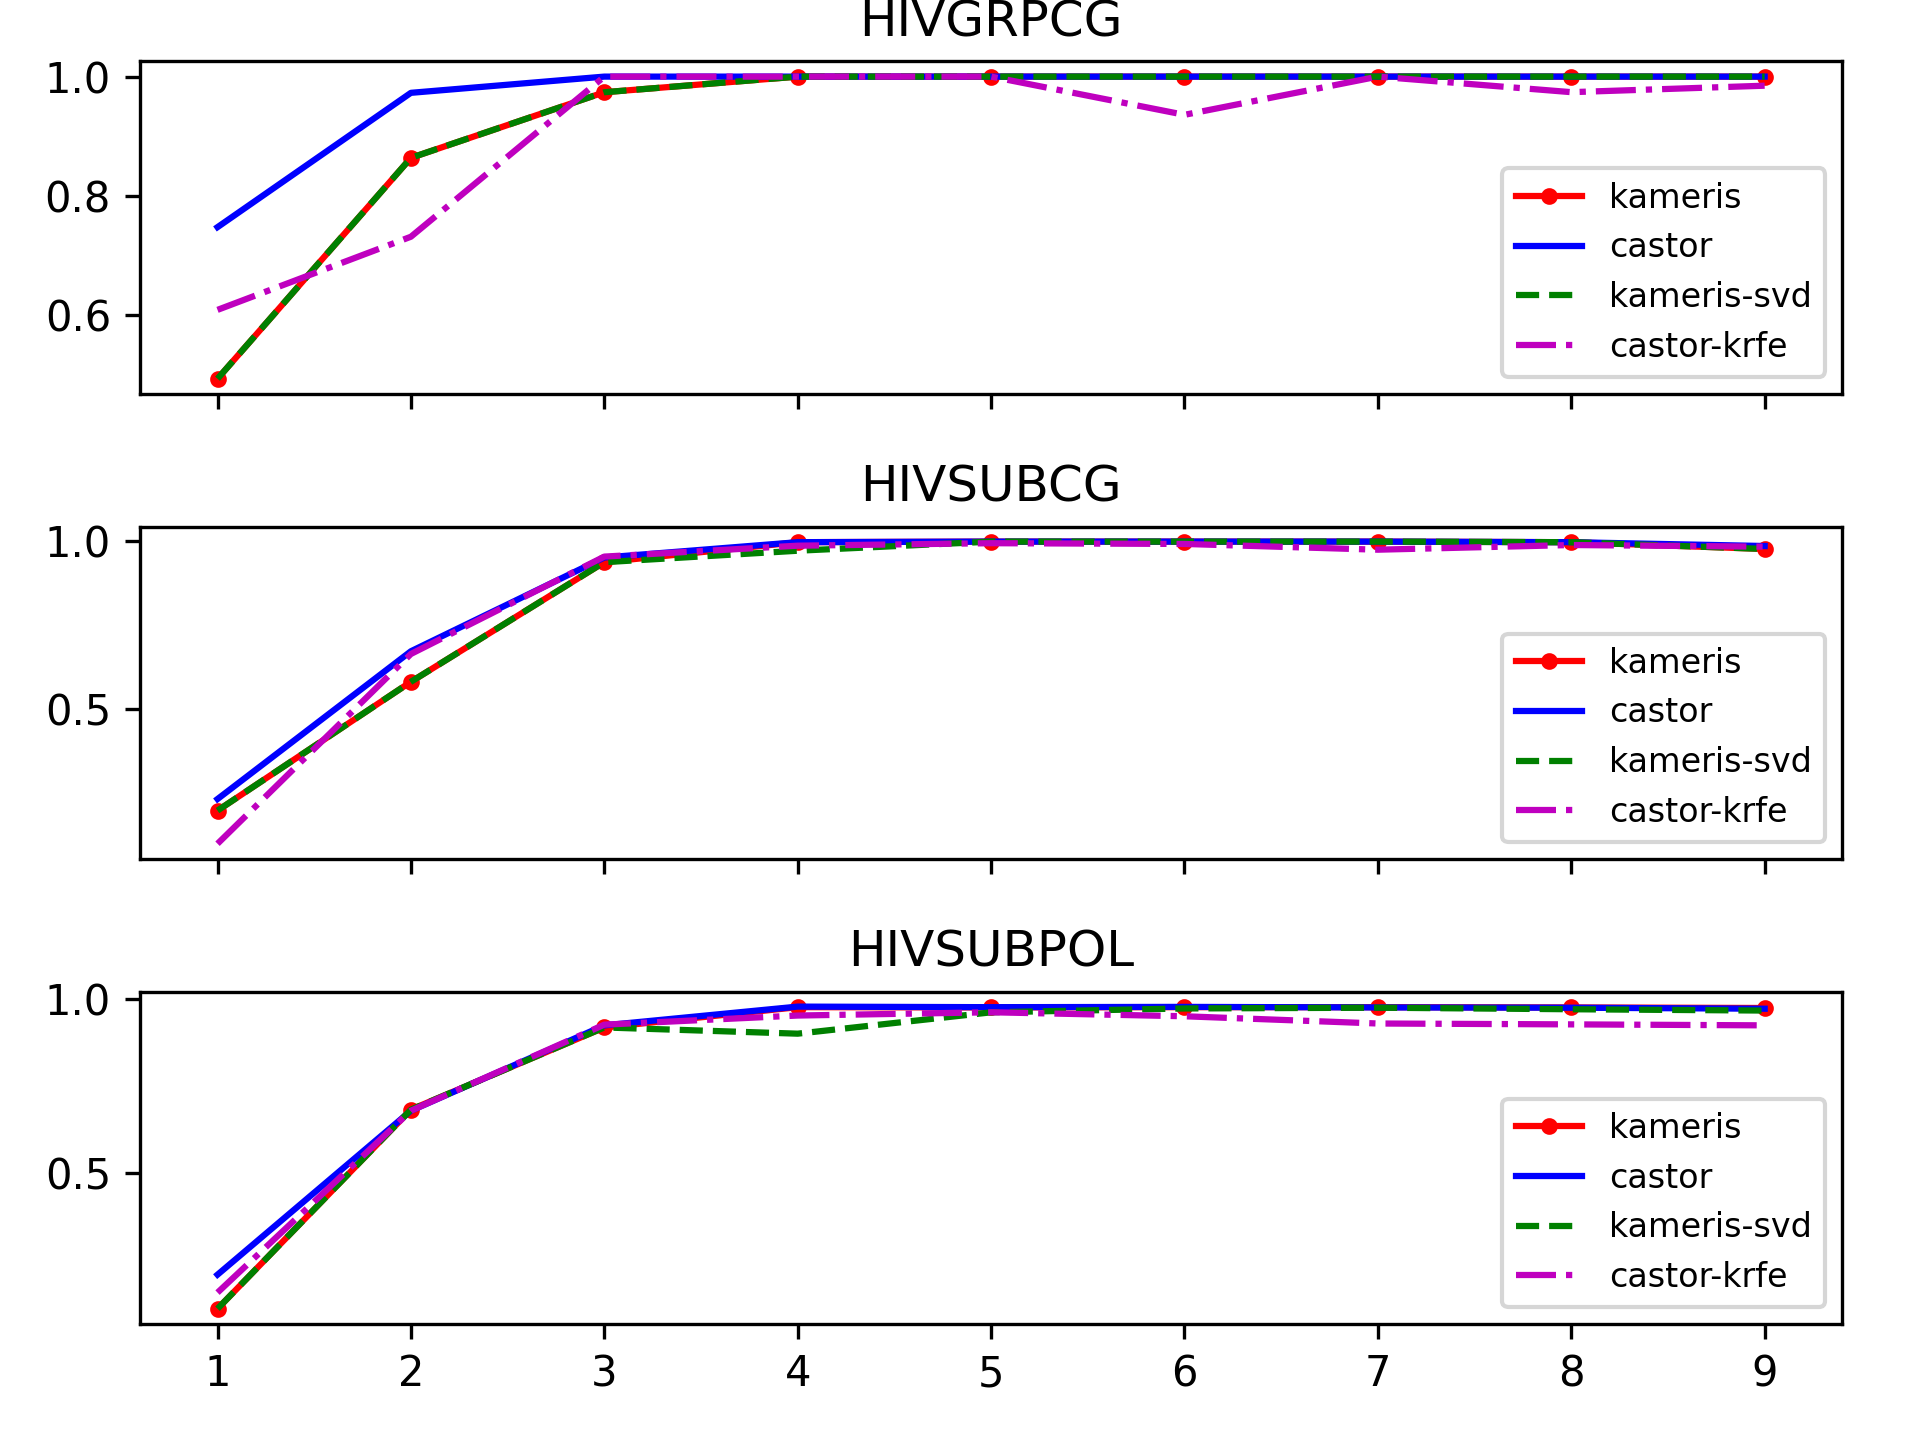
\includegraphics[width=0.7\textwidth]{img/kmer/comparison4_1_kameris_castor_dr=0_1}
		\caption{A comparison of f-score for the datasets HIVGRPCG, HIVSUBCG and HIVSUBPOL. The f-score were computed for different k-mers, ranging from k=1 to k=9. }
		\label{fig:comparison2}
	\end{figure}
	
\end{frame}
%-------------------------------------------------------
%-------------------------------------------------------


%-------------------------------------------------------
%-------------------------------------------------------
\begin{frame}{Results}{Vector size of Kameris and Castor}
	\begin{figure}[h]
		\centering
		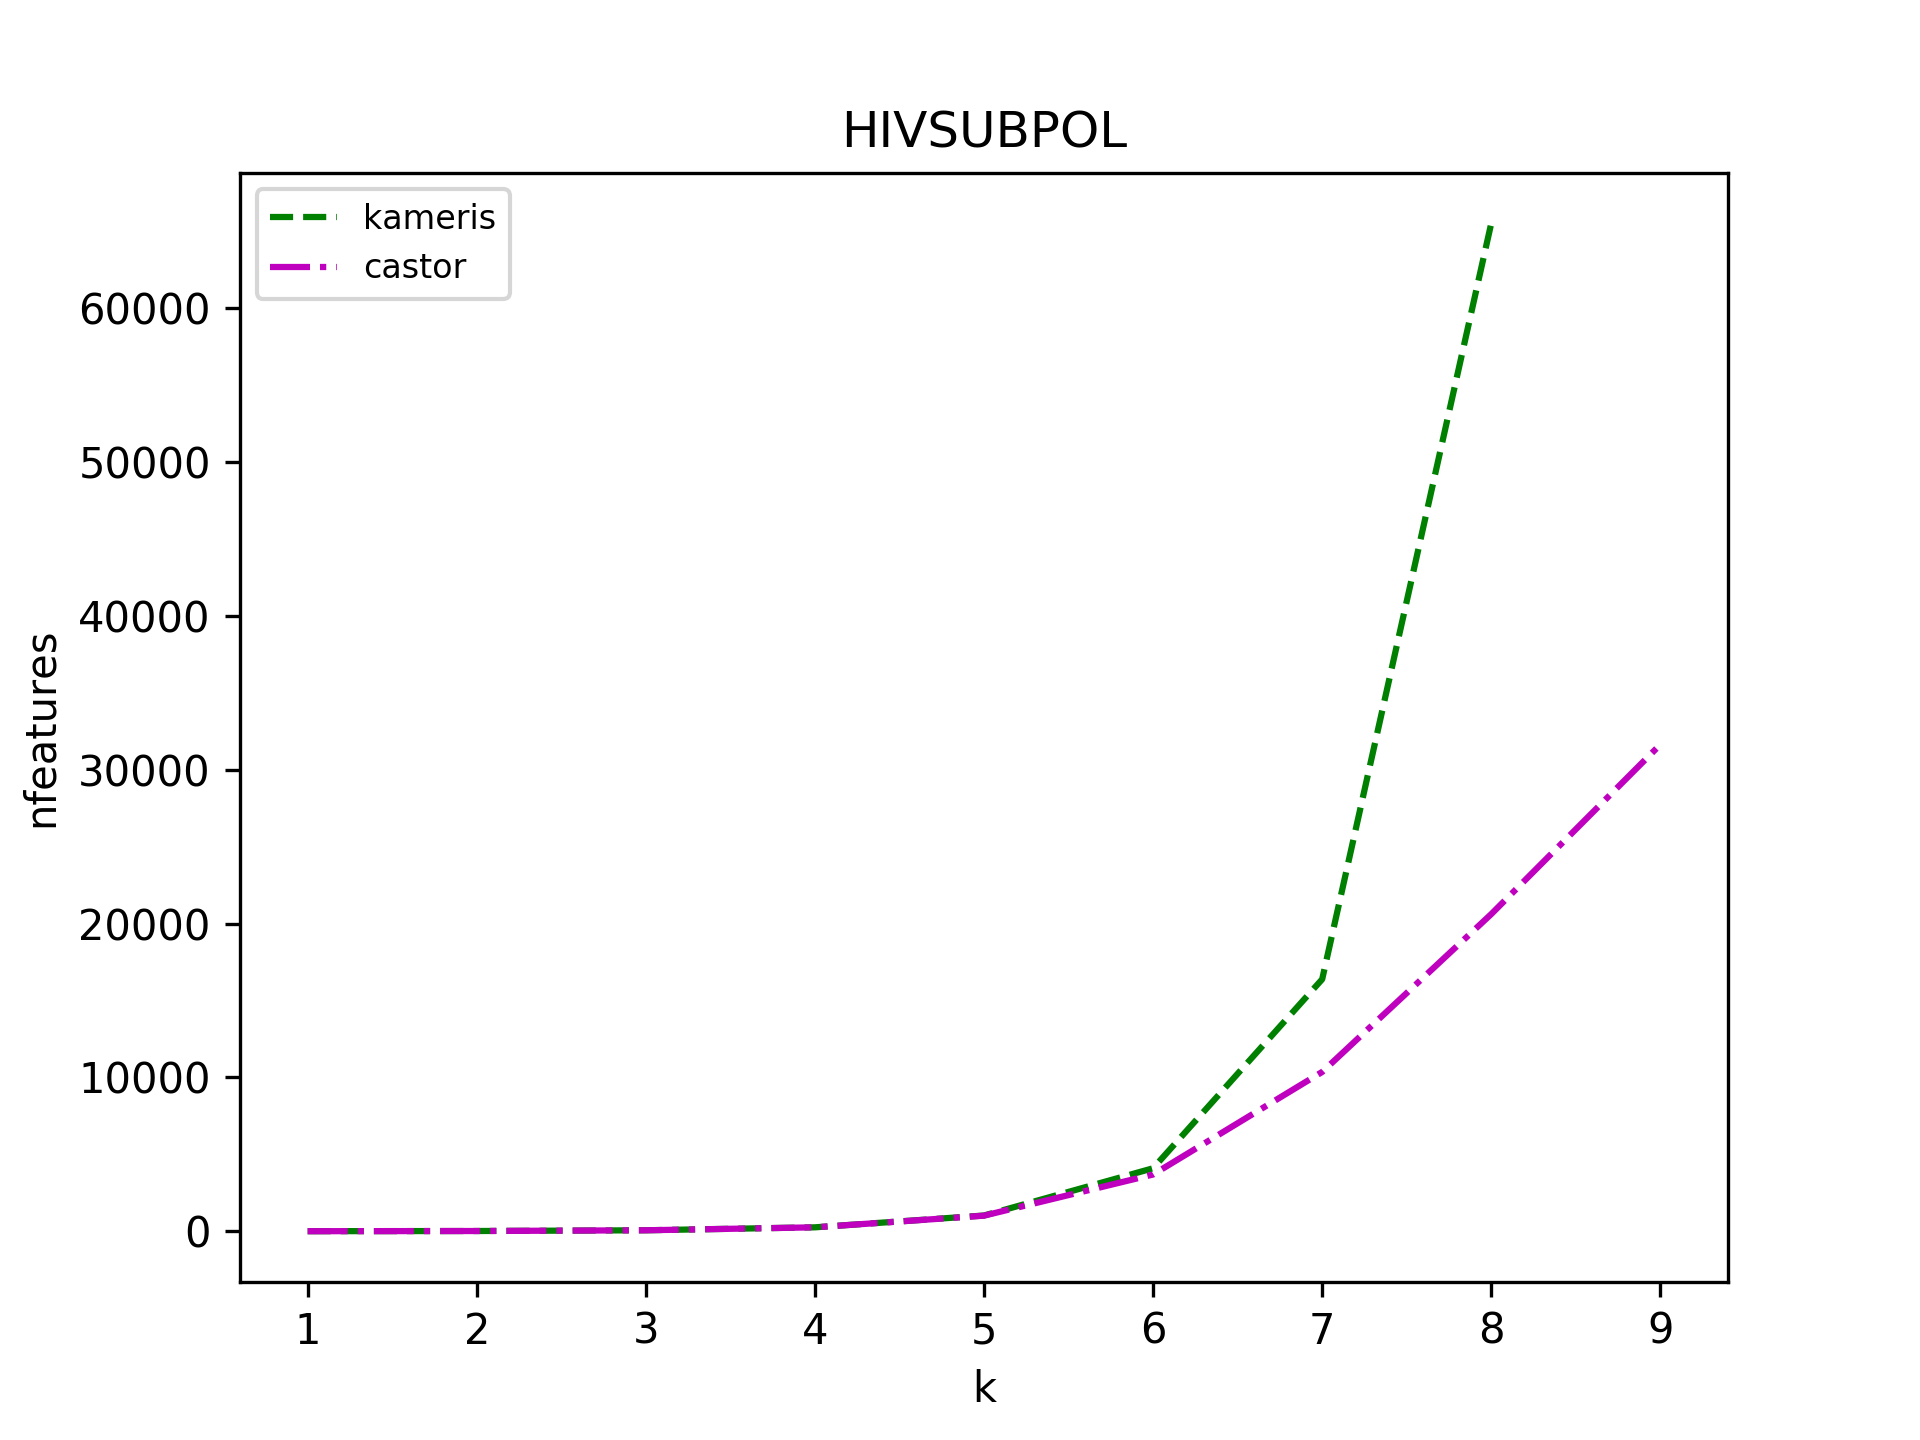
\includegraphics[width=0.7\textwidth]{img/kmer/comparison6_kameris_castor_dr=0.png}
		\caption{Size of feature vectors for Castor and Kameris without dimensionality SVD reduction and feature elimination RFE for  HIVSUBPOL dataset. X-axis represent $k$ value in k-mer.}
		\label{fig:comparison3}
	\end{figure}
	
\end{frame}
%-------------------------------------------------------
%-------------------------------------------------------


%-------------------------------------------------------
%-------------------------------------------------------
\begin{frame}{Results}{Vector size of Kameris and Castor}
	\begin{figure}[h]
		\centering
		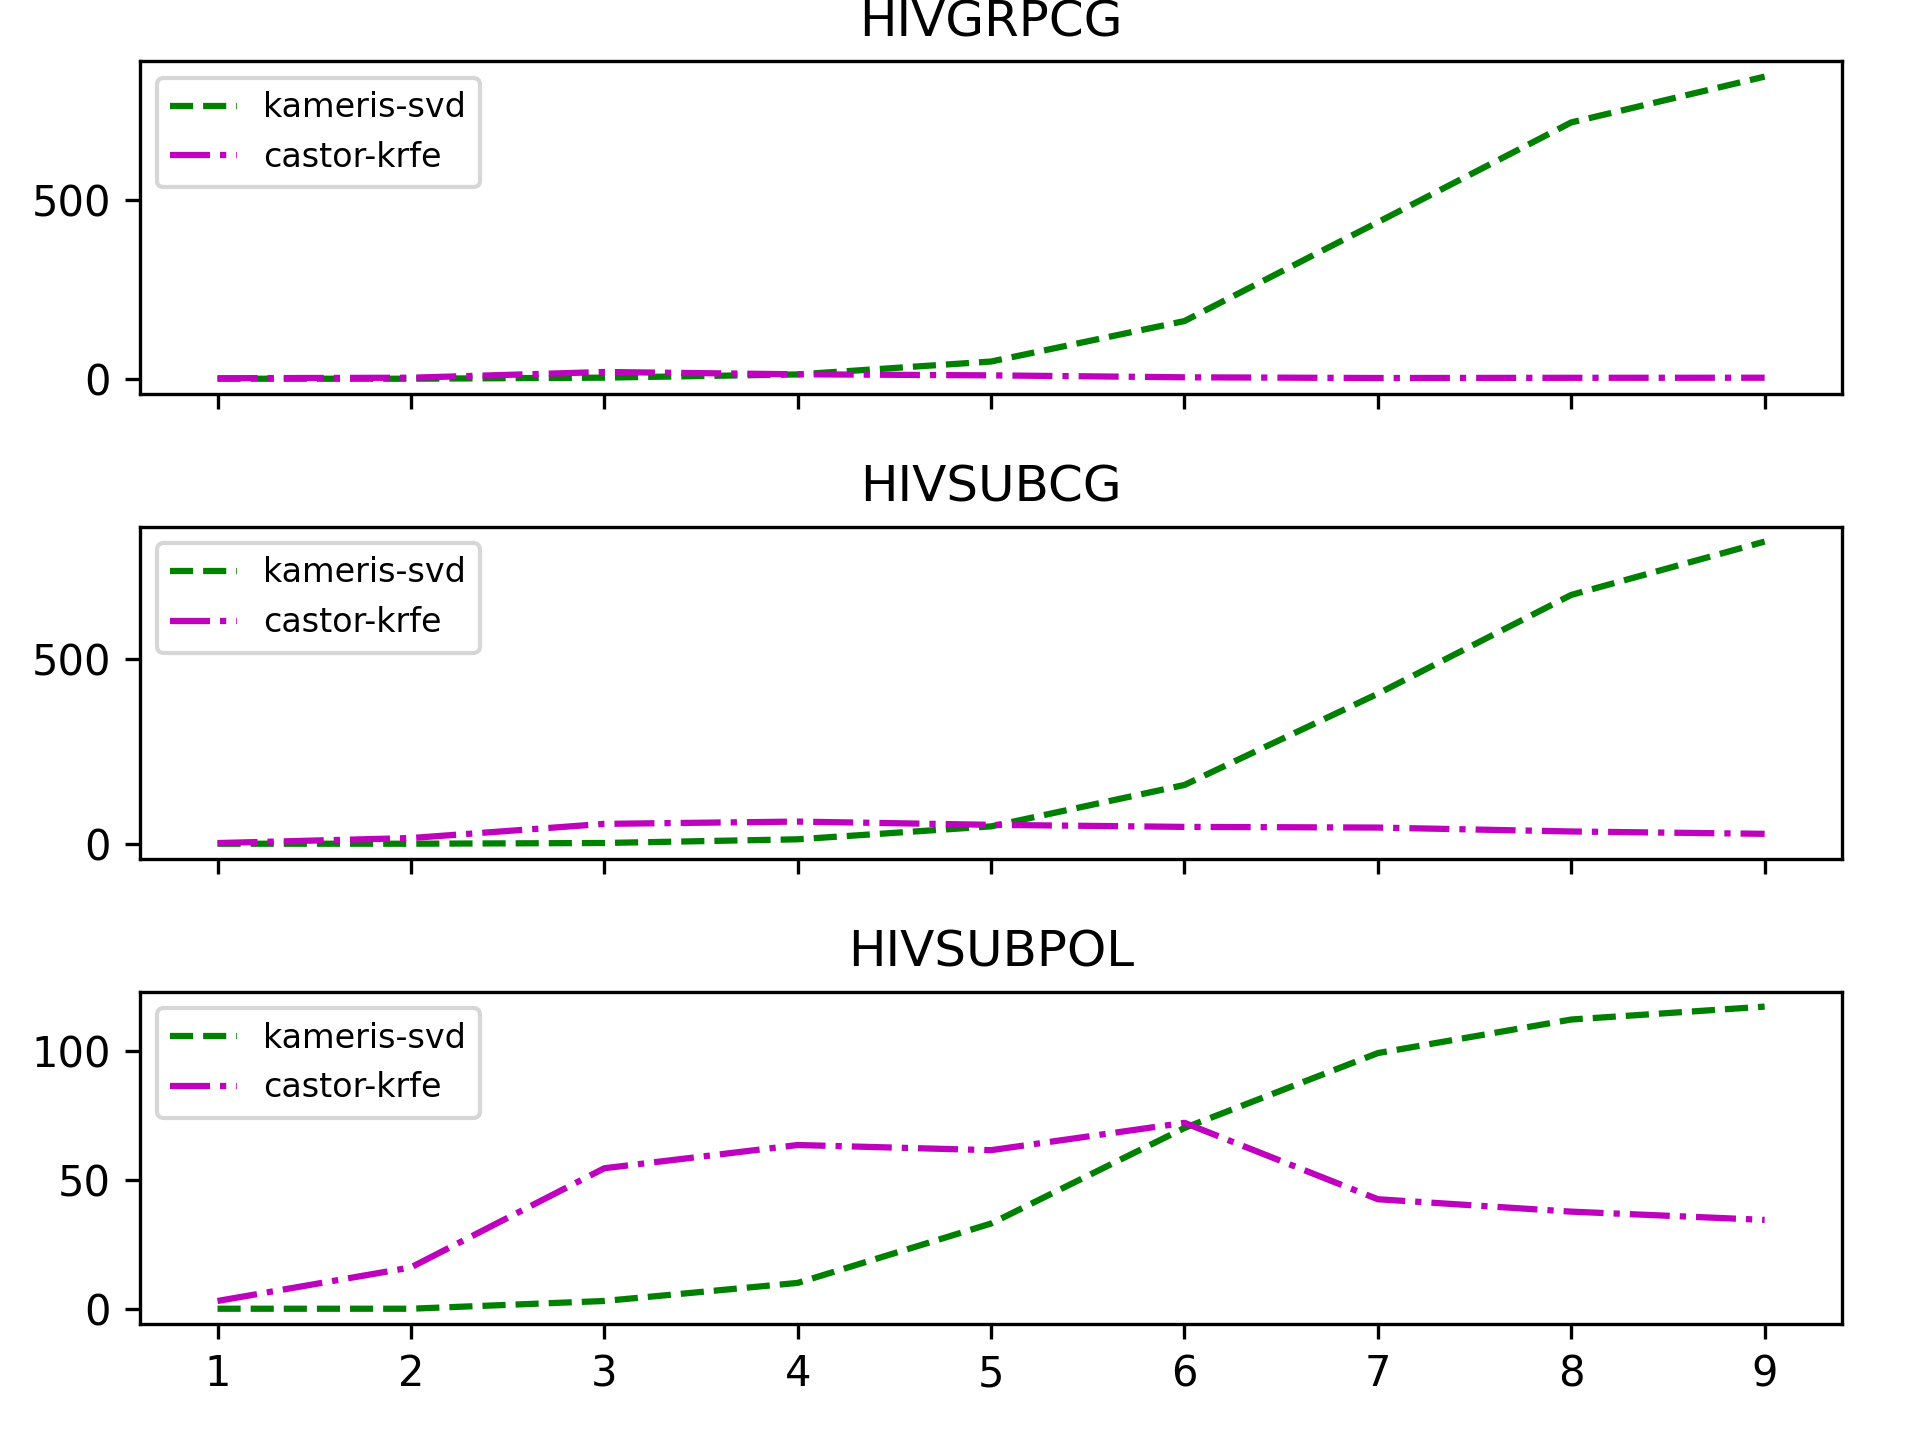
\includegraphics[width=0.7\textwidth]{img/kmer/comparison5_1_kameris_castor_dr=0_1.png}
		\caption{Size of feature vectors for Kameris-SVD/Kameris and Castor-KRFE/Castor for HIVGRPCG, HIVSUBCG and  HIVSUBPOL. X-axis represent $k$ value in k-mer.}
		\label{fig:comparison4}
	\end{figure}
	
\end{frame}
%-------------------------------------------------------
%-------------------------------------------------------


%-------------------------------------------------------
%-------------------------------------------------------
\begin{frame}{Results}{Kameris vs Castor}

\begin{table}[h]
	\begin{center}		
		\caption{The best f-score with the minimum $k$ value in k-mer by each dataset. Also, the number of features is presented.}
		\label{tab:results}
		\begin{tabular}{lccc}
			\hline			
			&	\multicolumn{3}{c}{Kameris-SVD}		       \\
			Dataset	&	(k-mer) 	& f-score     & nfeatures    \\				
			\hline
			
			HIVGRPCG  & 4 & 1.0000    & 12     \\
			HIVSUBCG  & 5 & \textbf{0.9983} & 47     \\
			HIVSUBPOL & 7 & \textbf{0.9761} & 99     \\
			
			& \multicolumn{3}{c}{Castor-KRFE}      \\
			Dataset	&	(k-mer) 	& f-score     & nfeatures    \\				
			\hline
			HIVGRPCG      & 3        & 1.0000   &   19 \\
			HIVSUBCG      & 5        & 0.9937   &   51 \\
			HIVSUBPOL     & 5        & 0.9629   &   65 \\
			
			\hline
		\end{tabular}		
		
	\end{center}
\end{table}
	
\end{frame}
%-------------------------------------------------------
%-------------------------------------------------------


%-------------------------------------------------------
%-------------------------------------------------------
\begin{frame}{Results}{Kameris, Castor, ML-DSP and CNN}
	
\begin{table}[]
	\centering
	\caption{Accuracy of the three CNN-2 architecture, ML-DSP, Kameris and Castor for each dataset.}
	\label{tab:acc_cnn_full}	
	\begin{tabular}{p{2cm}p{1.6cm}ccc}
		\hline
		Dataset          & ML-DSP & CNN-2 & Kameris       & Castor        \\ \hline
		EBOSPECG    & 0.92   & 1.00  & 1.00          & 1.00          \\
		HBVGENCG    & 0.15   & 1.00  & 1.00          & 1.00          \\
		HIVGRPCG    & 0.44   & 1.00  & 1.00          & 1.00          \\
		HIVSUBCG    & 0.05   & 0.98  & \textbf{1.00} & \textbf{1.00} \\
		HIVSUBPOL   & 0.01   & 0.97  & \textbf{1.00} & \textbf{1.00} \\
		INFSUBHA    & 1.00   & 1.00  & 1.00          & 1.00          \\
		INFSUBMP    & 0.89   & 0.98  & \textbf{0.99} & \textbf{0.99} \\
		INSUBFNA    & 1.00   & 1.00  & 1.00          & 1.00          \\
		RHISPECG    & 1.00   & 1.00  & 1.00          & 1.00          \\
		HPVGENCG    & 0.36   & 1.00  & 1.00          & 1.00          \\ \hline
		
	\end{tabular}
\end{table}
	
\end{frame}
%-------------------------------------------------------
%-------------------------------------------------------


%-------------------------------------------------------
%-------------------------------------------------------
\begin{frame}{Results}{Kameris, Castor, ML-DSP and CNN}
	
	\begin{table}[]
		\centering
		\caption{Accuracy of the three CNN-2 architecture, ML-DSP, Kameris and Castor for each dataset.}
		\label{tab:acc_cnn_full}	
		\begin{tabular}{p{2cm}p{1.6cm}ccc}
			\hline
			Dataset          & ML-DSP & CNN-2 & Kameris       & Castor        \\ \hline			
			Primates    & 0.97   & 1.00  & 1.00          & 1.00          \\
			Dengue      & 1.00   & 1.00  & 1.00          & 1.00          \\
			Protists    & 0.50   & 0.97  & \textbf{1.00} & \textbf{1.00} \\
			Fungi       & 0.40   & 1.00  & 1.00          & 1.00          \\
			Plants      & 0.69   & 0.91  & 0.89          & \textbf{0.97} \\
			Amphibians  & 0.60   & 1.00  & 1.00          & 1.00          \\
			Insects     & 0.37   & 0.97  & \textbf{0.99} & \textbf{0.99} \\
			3classes    & 0.57   & 1.00  & 1.00          & 1.00          \\
			Vertebrates & 0.52   & 1.00  & 1.00          & 1.00         \\ \hline
		\end{tabular}
	\end{table}
	
\end{frame}
%-------------------------------------------------------
%-------------------------------------------------------


%%%%%%%%%%%%%%%%%%%%%%%%%%%%%%%%%%%%%%%%%%%%%%%%%%%%%%%%
\section{Results}
%%%%%%%%%%%%%%%%%%%%%%%%%%%%%%%%%%%%%%%%%%%%%%%%%%%%%%%%

%-------------------------------------------------------
%-------------------------------------------------------
\begin{frame}{Results}{Kameris, Castor, ML-DSP and CNN}
	
	\begin{block}{}
		We evaluated four methods for viral subtyping classification, based on alignment-free algorithms.
	\end{block}

	\begin{block}{}
		Kameris-SVD outperformed slightly Castor-KRFE. Moreover, if we did not use SVD and RFE for each method, they got the same f1-score. 
	\end{block}

	\begin{block}{}
		 Castor-KRFE got a smaller feature vector than Kameris-SVD
	\end{block}

	\begin{block}{}
		Kameris and Castor without SVD and RFE got the best accuracy, but they are followed CNNs.
	\end{block}
	
\end{frame}
%-------------------------------------------------------
%-------------------------------------------------------


%-------------------------------------------------------
%-------------------------------------------------------
%\begin{frame}{CNN}{CNN model}
%	\begin{figure}[h]
%		\centering
%		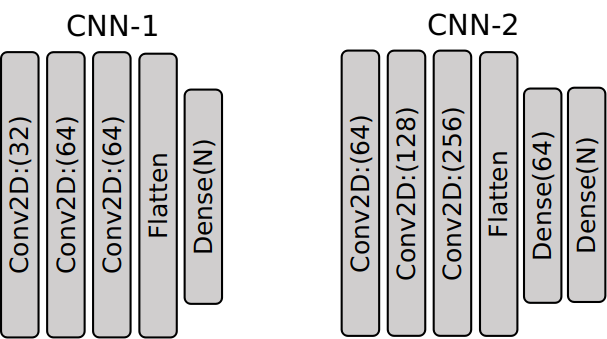
\includegraphics[width=0.3\textwidth]{img/kmer/cnn2}
%		\caption{CNN's architecture proposed.}
%		\label{fig:cnn}
%	\end{figure}
%\end{frame}
%-------------------------------------------------------
%-------------------------------------------------------

%-------------------------------------------------------
%-------------------------------------------------------
%\begin{frame}{CNN}{CNN model}
%	\begin{figure}[h]
%		\centering
%		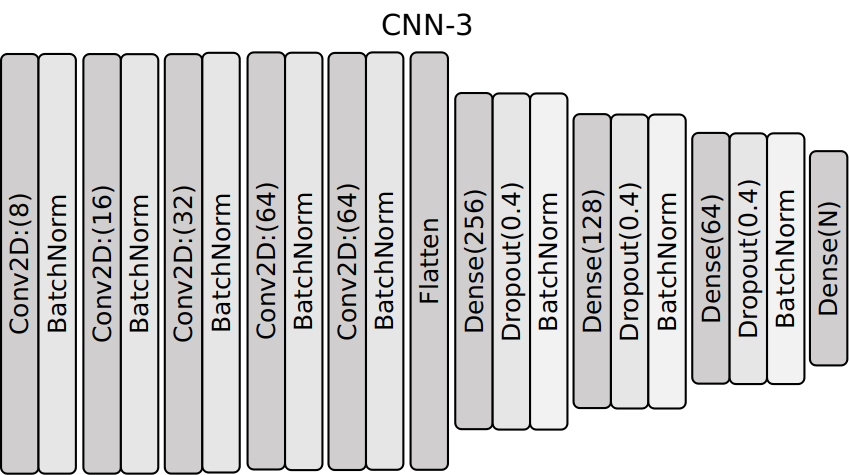
\includegraphics[width=0.45\textwidth]{img/kmer/cnn}
%		\caption{CNN's architecture proposed.}
%		\label{fig:cnn3}
%	\end{figure}
%\end{frame}
%-------------------------------------------------------
%-------------------------------------------------------



%-------------------------------------------------------
%-------------------------------------------------------
\begin{frame}[allowframebreaks]
	\frametitle{References}
	%\bibliographystyle{amsalpha}
	\bibliographystyle{IEEEtran}
	\bibliography{bibliography.bib}
\end{frame}
%-------------------------------------------------------
%-------------------------------------------------------



%-------------------------------------------------------
%-------------------------------------------------------
\if\mycmd1 % MY THEME
\1{
	{\1
		\begin{frame}[plain,noframenumbering]
			%\finalpage{Thank you}
			\begin{figure}[]
				\centering
				
\includegraphics[width=\textwidth,height=0.7\textheight,keepaspectratio]{img/question.png}
				%\label{img:mot2}
				%\caption{Image example in 2 gray levels.}
			\end{figure}
	\end{frame}}
	\else % CS THEME
	\begin{frame}{Questions?}
		\begin{figure}[]
			\centering
			
\includegraphics[width=\textwidth,height=0.7\textheight,keepaspectratio]{img/question.png}
			%\label{img:mot2}
			%\caption{Image example in 2 gray levels.}
		\end{figure}
		
	\end{frame}
	\fi
	%-------------------------------------------------------
	%-------------------------------------------------------
	

\end{document}